
\documentclass[border={7pt 0pt 90pt 0pt},varwidth]{standalone}
\usepackage{amsmath}
\usepackage{tikz-cd,tikz-3dplot} 
\usepackage{quiver}
\usepackage{diagbox}
\usepackage{xcolor}%colors
\usepackage{makecell}
\usepackage{adjustbox}
\usepackage[width=0.5,tiewidth=0.7]{strands}
\usetikzlibrary{calc,intersections,through,backgrounds,decorations.pathmorphing, decorations.shapes,decorations.markings,patterns}
%include other needed packages here   

\DeclareMathOperator{\GL}{\operatorname{GL}}
\DeclareMathOperator{\SL}{\operatorname{SL}}
\DeclareMathOperator{\supp}{supp}
\DeclareMathOperator{\dist}{dist}
\DeclareMathOperator{\vol}{vol}
\DeclareMathOperator{\diag}{diag}
\DeclareMathOperator{\tr}{tr}
\DeclareMathOperator{\Img}{\operatorname{Im}}
\DeclareMathOperator{\Id}{\operatorname{Id}}
\DeclareMathOperator{\rep}{\operatorname{rep}}
\DeclareMathOperator{\Rep}{\operatorname{Rep}}
\DeclareMathOperator{\RRep}{\widetilde{\operatorname{Rep}}}
\DeclareMathOperator{\Mod}{\operatorname{Mod}}
\DeclareMathOperator{\Hom}{\operatorname{Hom}}
\DeclareMathOperator{\Ext}{\operatorname{Ext}}
\DeclareMathOperator{\gldim}{\operatorname{gl.dim}}
\DeclareMathOperator{\projdim}{\operatorname{proj.dim}}
\DeclareMathOperator{\injdim}{\operatorname{inj.dim}}
\DeclareMathOperator{\dimv}{\operatorname{\underline{\mathbf{dim}}}}
\DeclareMathOperator{\Pic}{\operatorname{Pic}}
\DeclareMathOperator{\Jac}{\operatorname{Jac}}
\DeclareMathOperator{\ptt}{\operatorname{par}}
\newcommand{\Spec}{\operatorname{Spec}}
\DeclareMathOperator{\St}{\mathcal{Z}}
\DeclareMathOperator{\Flagd}{\operatorname{Flag}_{\mathbf{d}}}
\DeclareMathOperator{\Flagdstr}{\operatorname{Flag}_{\mathbf{d},str}}
\newcommand{\Gr}{\operatorname{Gr}}
\newcommand{\Grr}{\operatorname{Gr}}
\newcommand{\Grq}{\operatorname{Gr}^{KQ}}
\newcommand{\Flag}[1]{\operatorname{Flag}_{\mathbf{#1}}}
\newcommand{\Flagstr}[1]{\operatorname{Flag}_{\mathbf{#1},str}}
\newcommand{\dimvec}[1]{\mathbf{#1}}
\newcommand{\abdimvec}[1]{|\dimvec{#1}|}
\newcommand{\ftdimvec}[1]{\underline{\dimvec{#1}}}
\newcommand{\absgp}[1]{\mathbb{#1}}
\newcommand{\ww}{\varpi}
\DeclareMathOperator{\MinWd}{\operatorname{Min}(\absgp{W}_{\abdimvec{d}},W_{\dimvec{d}})}
\DeclareMathOperator{\Compd}{\operatorname{Comp}_{\dimvec{d}}}
\DeclareMathOperator{\Shuffled}{\operatorname{Schuffle}_{\dimvec{d}}}
\newcommand{\WWd}{\absgp{W}_{\abdimvec{d}}}
\newcommand{\Wd}{W_{\dimvec{d}}}

\newcommand{\Omcell}{\Omega}
\newcommand{\OOmcell}{\boldsymbol{\Omega}}
\newcommand{\Vcell}{\mathcal{V}}
\newcommand{\VVcell}{\boldsymbol{\mathcal{V}}}
\newcommand{\Ocell}{\mathcal{O}}
\newcommand{\OOcell}{\boldsymbol{\mathcal{O}}}

%\newcommand{\lbox}{\adjustbox{cfbox=red, margin=-\fboxrule-\fboxsep}}
\newcommand{\lbox}{\adjustbox{}}

\newenvironment{smbmatrix}% environment name
{% begin code
\bgroup
\setlength\arraycolsep{1pt}
\renewcommand{\arraystretch}{0.6}
\setcellgapes{0.2ex}
  \begin{bmatrix}
}%
{\end{bmatrix}
\egroup
}% end code
\newenvironment{smpmatrix}% environment name
{% begin code
\bgroup
\setlength\arraycolsep{1pt}
\renewcommand{\arraystretch}{0.8}
\setcellgapes{0.2ex}
  \begin{pmatrix}
}%
{\end{pmatrix}
\egroup
}% end code

\makeatletter
\renewcommand*\env@matrix[1][*\c@MaxMatrixCols c]{%
  \hskip -\arraycolsep
  \let\@ifnextchar\new@ifnextchar
  \array{#1}}
\makeatother
\begin{document}

\begin{table}[ht]
 \[
 \setcellgapes{0.8ex}\makegapedcells
 \begin{array}{|c|c|ccc|ccc|}
 \hline
 &&\mathfrak{n}_u&\mathfrak{m}_{u,u}&&\mathfrak{r}_u&\mathfrak{d}_{u,u}&\\\hline
 &u\phantom{s_1}=\parbox[h][][c]{1.5cm}{
  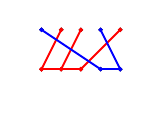
\begin{tikzpicture}[scale=0.5]
  \vpartition[
  floor=0,
  tkzpic=0,
  type=0
  ]{{5}}
  \tie[color=red,bull=1,bulletie=0.04,style=solid,tieheight=0]{{1},{2},{3}}
  \tie[color=red,bull=1,bulletie=0.04,style=solid]{{2,1},{1,0}}
  \tie[color=red,bull=1,bulletie=0.04,style=solid]{{3,1},{2,0}}
  \tie[color=red,bull=1,bulletie=0.04,style=solid]{{5,1},{3,0}}
  \tie[color=blue,bull=1,bulletie=0.04,style=solid]{{1,1},{4,0},{5,0},{4,1}}
  \end{tikzpicture}
  }\phantom{\in \Wd u} &
  \begin{smbmatrix}[ccc|cc]
\phantom{*}&*&*&&\\
&\phantom{*}&*&&\\
&&\phantom{*}&&\\\hline
&&&\phantom{*}&*\\
&&&&\phantom{*}\\
\end{smbmatrix}
&
  \begin{smbmatrix}[ccc|cc]
\phantom{*}&&&&\\
&\phantom{*}&&&\\
&&\phantom{*}&&\\\hline
&&&\phantom{*}&\\
&&&&\phantom{*}\\
\end{smbmatrix}
&&
  \begin{smbmatrix}[ccc|cc]
\phantom{*}&&&&\\
&\phantom{*}&&&\\
&&\phantom{*}&&\\\hline
*&*&*&\phantom{*}&\\
&&*&&\phantom{*}\\
\end{smbmatrix}
&
  \begin{smbmatrix}[ccc|cc]
\phantom{*}&&&&\\
&\phantom{*}&&&\\
&&\phantom{*}&&\\\hline
&&&\phantom{*}&\\
&&&&\phantom{*}\\
\end{smbmatrix}&
 \\\hline
  s&\text{cases}&\mathfrak{n}_{us}&\mathfrak{m}_{u,us}&&\mathfrak{r}_{us}&\mathfrak{d}_{u,us}&\\\hline
 
 s=s_1&us_1=\parbox[h][][c]{1.5cm}{
   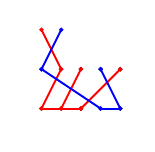
\begin{tikzpicture}[scale=0.5]
   \vpartition[
   floor=0,
   tkzpic=0,
   type=0
   ]{{5}}
   \tie[color=red,bull=1,bulletie=0.04,style=solid,tieheight=0]{{1},{2},{3}}
   \tie[color=red,bull=1,bulletie=0.04,style=solid]{{1,2},{2,1},{1,0}}
   \tie[color=red,bull=1,bulletie=0.04,style=solid]{{3,1},{2,0}}
   \tie[color=red,bull=1,bulletie=0.04,style=solid]{{5,1},{3,0}}
   \tie[color=blue,bull=1,bulletie=0.04,style=solid]{{2,2},{1,1},{4,0},{5,0},{4,1}}
   \end{tikzpicture}
   }\notin \Wd u &
   \begin{smbmatrix}[ccc|cc]
 \phantom{*}&*&*&&\\
 &\phantom{*}&*&&\\
 &&\phantom{*}&&\\\hline
 &&&\phantom{*}&*\\
 &&&&\phantom{*}\\
 \end{smbmatrix}
 &
   \begin{smbmatrix}[ccc|cc]
 \phantom{*}&&&&\\
 &\phantom{*}&&&\\
 &&\phantom{*}&&\\\hline
 &&&\phantom{*}&\\
 &&&&\phantom{*}\\
 \end{smbmatrix}
 &&
   \begin{smbmatrix}[ccc|cc]
\phantom{*}&&&&\\
&\phantom{*}&&&\\
&&\phantom{*}&&\\\hline
&*&*&\phantom{*}&\\
&&*&&\phantom{*}\\
 \end{smbmatrix}
 &
   \begin{smbmatrix}[ccc|cc]
 \phantom{*}&&&&\\
 &\phantom{*}&&&\\
 &&\phantom{*}&&\\\hline
 *&&&\phantom{*}&\\
 &&&&\phantom{*}\\
 \end{smbmatrix}& {\displaystyle\frac{e_4}{e_1}}
  \\\hline
  
  s=s_2&us_2=\parbox[h][][c]{1.5cm}{
    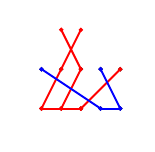
\begin{tikzpicture}[scale=0.5]
    \vpartition[
    floor=0,
    tkzpic=0,
    type=0
    ]{{5}}
    \tie[color=red,bull=1,bulletie=0.04,style=solid,tieheight=0]{{1},{2},{3}}
    \tie[color=red,bull=1,bulletie=0.04,style=solid]{{3,2},{2,1},{1,0}}
    \tie[color=red,bull=1,bulletie=0.04,style=solid]{{2,2},{3,1},{2,0}}
    \tie[color=red,bull=1,bulletie=0.04,style=solid]{{5,1},{3,0}}
    \tie[color=blue,bull=1,bulletie=0.04,style=solid]{{1,1},{4,0},{5,0},{4,1}}
    \end{tikzpicture}
    }\in \Wd u &
    \begin{smbmatrix}[ccc|cc]
  \phantom{*}&&*&&\\
  *&\phantom{*}&*&&\\
  &&\phantom{*}&&\\\hline
  &&&\phantom{*}&*\\
  &&&&\phantom{*}\\
  \end{smbmatrix}
  &
    \begin{smbmatrix}[ccc|cc]
  \phantom{*}&*&&&\\
  &\phantom{*}&&&\\
  &&\phantom{*}&&\\\hline
  &&&\phantom{*}&\\
  &&&&\phantom{*}\\
  \end{smbmatrix}
  &{\displaystyle\frac{e_1}{e_2}}&
    \begin{smbmatrix}[ccc|cc]
\phantom{*}&&&&\\
&\phantom{*}&&&\\
&&\phantom{*}&&\\\hline
*&*&*&\phantom{*}&\\
&&*&&\phantom{*}\\
  \end{smbmatrix}
  &
    \begin{smbmatrix}[ccc|cc]
  \phantom{*}&&&&\\
  &\phantom{*}&&&\\
  &&\phantom{*}&&\\\hline
  &&&\phantom{*}&\\
  &&&&\phantom{*}\\
  \end{smbmatrix}&
   \\\hline
   
   s=s_3&us_3=\parbox[h][][c]{1.5cm}{
     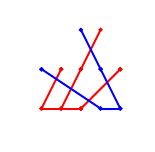
\begin{tikzpicture}[scale=0.5]
     \vpartition[
     floor=0,
     tkzpic=0,
     type=0
     ]{{5}}
     \tie[color=red,bull=1,bulletie=0.04,style=solid,tieheight=0]{{1},{2},{3}}
     \tie[color=red,bull=1,bulletie=0.04,style=solid]{{2,1},{1,0}}
     \tie[color=red,bull=1,bulletie=0.04,style=solid]{{4,2},{3,1},{2,0}}
     \tie[color=red,bull=1,bulletie=0.04,style=solid]{{5,1},{3,0}}
     \tie[color=blue,bull=1,bulletie=0.04,style=solid]{{1,1},{4,0},{5,0},{4,1},{3,2}}
     \end{tikzpicture}
     }\notin \Wd u &
     \begin{smbmatrix}[ccc|cc]
   \phantom{*}&*&*&&\\
   &\phantom{*}&*&&\\
   &&\phantom{*}&&\\\hline
   &&&\phantom{*}&*\\
   &&&&\phantom{*}\\
   \end{smbmatrix}
   &
     \begin{smbmatrix}[ccc|cc]
   \phantom{*}&&&&\\
   &\phantom{*}&&&\\
   &&\phantom{*}&&\\\hline
   &&&\phantom{*}&\\
   &&&&\phantom{*}\\
   \end{smbmatrix}
   &&
     \begin{smbmatrix}[ccc|cc]
\phantom{*}&&&&\\
&\phantom{*}&&&\\
&&\phantom{*}&&\\\hline
*&*&*&\phantom{*}&\\
&*&*&&\phantom{*}\\
   \end{smbmatrix}
   &
     \begin{smbmatrix}[ccc|cc]
   \phantom{*}&&&&\\
   &\phantom{*}&&&\\
   &&\phantom{*}&&\\\hline
   &&&\phantom{*}&\\
   &&&&\phantom{*}\\
   \end{smbmatrix}&
    \\\hline
    
 s=s_4&us_4=\parbox[h][][c]{1.5cm}{
   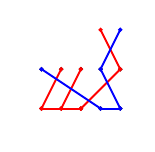
\begin{tikzpicture}[scale=0.5]
   \vpartition[
   floor=0,
   tkzpic=0,
   type=0
   ]{{5}}
   \tie[color=red,bull=1,bulletie=0.04,style=solid,tieheight=0]{{1},{2},{3}}
   \tie[color=red,bull=1,bulletie=0.04,style=solid]{{2,1},{1,0}}
   \tie[color=red,bull=1,bulletie=0.04,style=solid]{{3,1},{2,0}}
   \tie[color=red,bull=1,bulletie=0.04,style=solid]{{4,2},{5,1},{3,0}}
   \tie[color=blue,bull=1,bulletie=0.04,style=solid]{{1,1},{4,0},{5,0},{4,1},{5,2}}
   \end{tikzpicture}
   }\notin \Wd u &
   \begin{smbmatrix}[ccc|cc]
   \phantom{*}&*&*&&\\
   &\phantom{*}&*&&\\
   &&\phantom{*}&&\\\hline
   &&&\phantom{*}&*\\
   &&&&\phantom{*}\\
 \end{smbmatrix}
 &
   \begin{smbmatrix}[ccc|cc]
 \phantom{*}&&&&\\
 &\phantom{*}&&&\\
 &&\phantom{*}&&\\\hline
 &&&\phantom{*}&\\
 &&&&\phantom{*}\\
 \end{smbmatrix}
 &&
   \begin{smbmatrix}[ccc|cc]
\phantom{*}&&&&\\
&\phantom{*}&&&\\
&&\phantom{*}&&\\\hline
*&*&*&\phantom{*}&\\
&&&&\phantom{*}\\
 \end{smbmatrix}
 &
   \begin{smbmatrix}[ccc|cc]
 \phantom{*}&&&&\\
 &\phantom{*}&&&\\
 &&\phantom{*}&&\\\hline
 &&&\phantom{*}&\\
 &&*&&\phantom{*}\\
 \end{smbmatrix}& {\displaystyle\frac{e_5}{e_3}}
  \\\hline
 \end{array}
 \]
        
\end{table}
\end{document}